\section{Causas raíz}

La figura~\ref{fig:ishikawa} agrupa las causas en un diagrama de Ishikawa. La causa directa fue el comando de mantenimiento, pero no basta para explicar seis horas fuera de línea: la herramienta de auditoría que debía detener ese tipo de comandos tenía un error y lo dejó pasar \cite{meta_detalles}. Dos decisiones de diseño agrandaron el daño. Los servidores DNS se retiran solos cuando no ven los centros de datos, y como todos los perdieron a la vez, todos se retiraron. La red de acceso fuera de banda tampoco funcionó, así que los ingenieros tuvieron que ir en persona a los centros de datos, cuya seguridad física hizo más lenta la entrada \cite{meta_detalles}. No es un caso aislado: los errores de configuración están entre las causas dominantes de fallos en sistemas reales \cite{yin2011}.

\begin{figure}[h]
  \centering
  \IfFileExists{../diagrama/ishikawa.pdf}
    {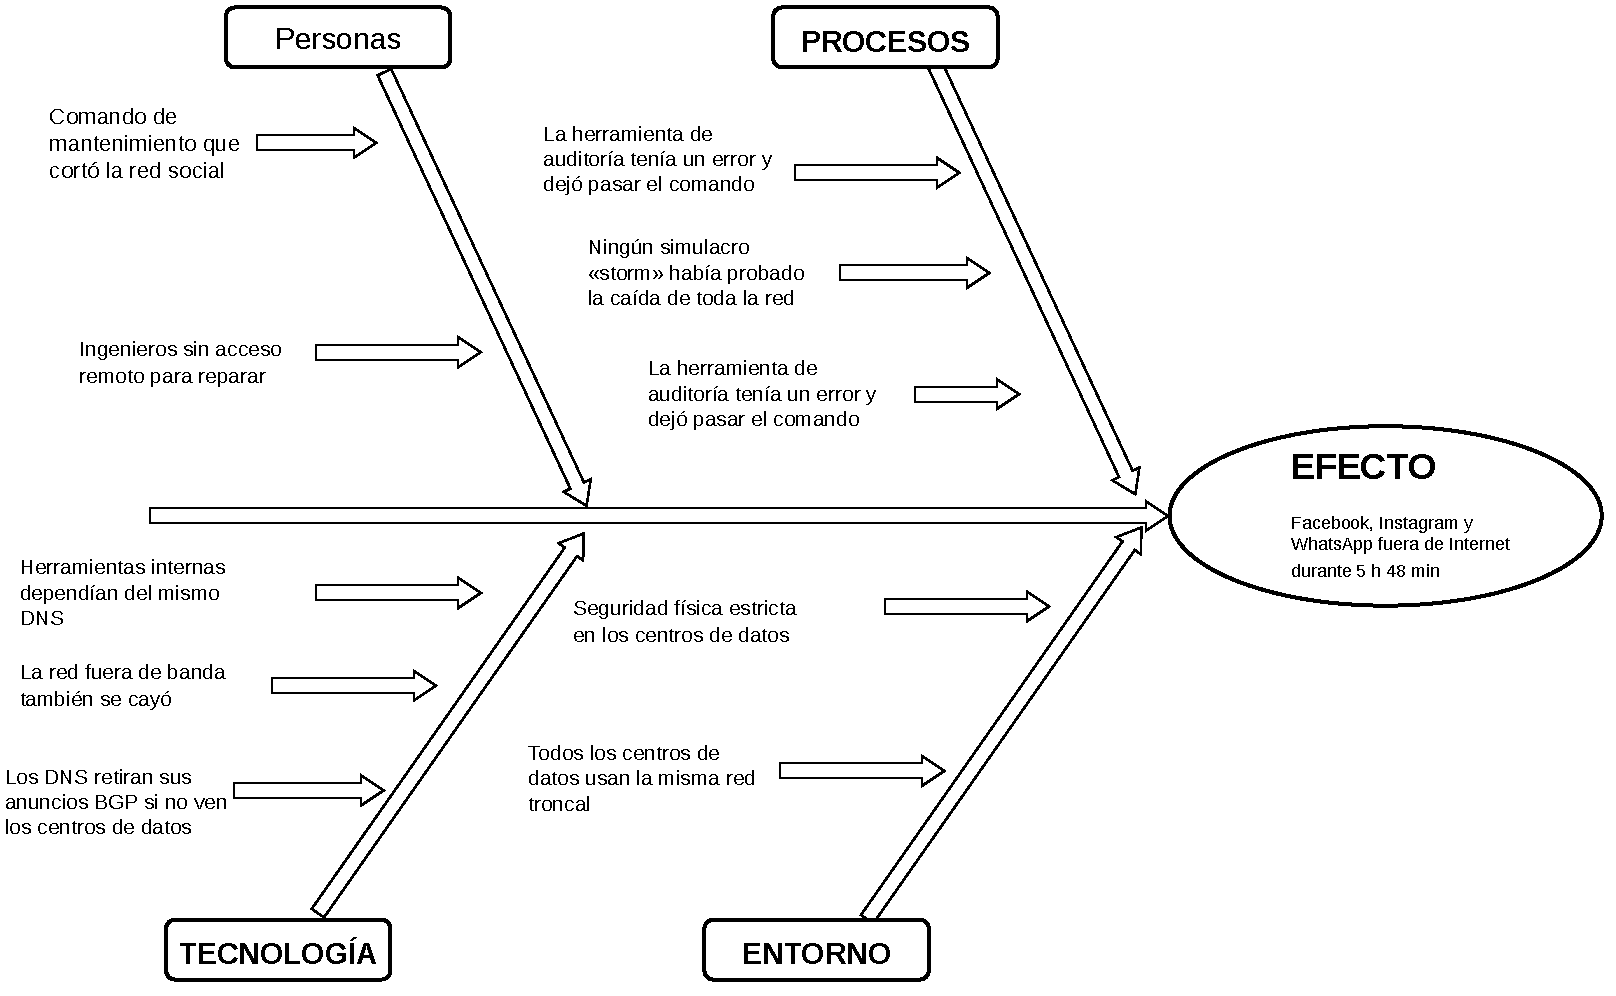
\includegraphics[width=\linewidth]{../diagrama/ishikawa.pdf}}
    {\IfFileExists{../diagrama/ishikawa.png}
      {\includegraphics[width=\linewidth]{../diagrama/ishikawa.png}}
      {\fbox{\parbox{0.9\linewidth}{\centering Falta \texttt{diagrama/ishikawa.pdf}.}}}}
  \caption{Diagrama de Ishikawa de la caída de Facebook, elaborado por el equipo en draw.io con base en \cite{meta_detalles,meta_actualizacion}.}
  \label{fig:ishikawa}
\end{figure}
